\documentclass[tikz,border=5pt]{standalone}
\usetikzlibrary{arrows.meta, calc}
\usepackage{bm}

\begin{document}
    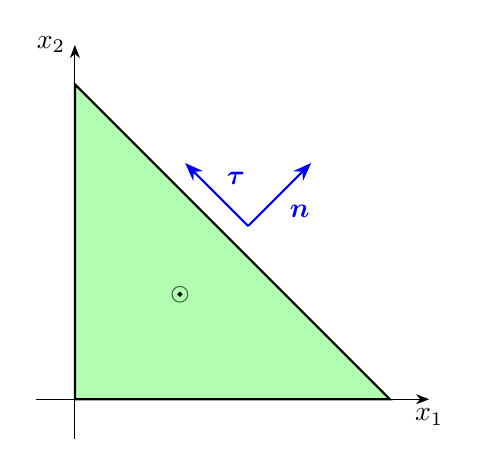
\begin{tikzpicture}[
        >=Stealth,
        dot/.style={circle, fill, inner sep=1.5pt},
        normal/.style={->, blue, thick},
        tangent/.style={->, blue, thick}
    ]

% Оси координат
        \draw[->] (-0.5,0) -- (4.5,0) node[below] {$x_1$};
        \draw[->] (0,-0.5) -- (0,4.5) node[left] {$x_2$};

% Равносторонний треугольник с катетами по осям
        \draw[fill=green!30, thick] (0,0) -- (4,0) -- (0,4) -- cycle;

% Гипотенуза и её середина
        \draw[dashed] (0,4) -- (4,0);
        \coordinate (midhyp) at (2,2); % середина гипотенузы

% Пересечение медиан (центроид)
        \coordinate (centroid) at (4/3, 4/3); % для треугольника с катетами длины 4

% Окружность в центроиде
        \draw[fill=green!30, opacity=0.6] (centroid) circle (0.1);

% Точка в центроиде
        \draw[fill=black] (centroid) circle (0.025);

% Точка около середины гипотенузы (снаружи)
        \coordinate (P) at ($(midhyp) + (0.2,0.2)$); % смещение 0.2 от середины наружу

% Векторы (исправленные направления)
% Внешняя нормаль: перпендикулярна гипотенузе и направлена наружу от треугольника
% Направление: от точки P вправо-вверх (наружу)
        \draw[normal] (P) -- ++(0.8,0.8) node[midway, below right] {$\bm{n}$};

% Касательная: перпендикулярна нормали, направлена вдоль гипотенузы
        \draw[tangent] (P) -- ++(-0.8,0.8) node[midway, above right] {$\bm{\tau}$};
    \end{tikzpicture}
\end{document}